% chap4.tex (Definitions and Theorem)

\chapter{Provenance Graphs size optimization using Graph Summarization} \label{MostNarrowEasy}

In this chapter, we explore optimization of provenance graph size using a graph summarization approach. 

%\section{A Policy-Based Approach for Provenance Storage}

\section{Introduction}

Data provenance captures information flow of across a systems which has applications in forensic analysis, intrusion detection and to scientific research for experiment reproducability. Due to the benefit it offers, provenance has received a significant amount of attention from the scientific community in recent years and has led to the development of various provenance-aware applications. For example, PASS \cite{muniswamy_reddy} and HiFi \cite{Bates2014LinuxPM}, both linux based provenance collection system which captures interaction between file level interactions and system calls. Chimera \cite{chimera} and myGrid,  a provenance collection system for scientific workflow reproducibility. 


However, one of the major challenge faced by provenance-aware systems is that provenance data incurs additional storage overhead. That is, provenance can easily generate more data than the data in which provenance is is being captured for. Our framework, PAIoT is no exception. Due to the large influx of real-time data generated from sensors and actuators, and preliminary results derived, we envision large amounts of provenance data generated from our provenance collection framework. The resource constraints on the sensor-actuator and the device layer of the IoT architecture makes storing this data a more challenging task. Motivated by the need to provide an efficient provenance record, we address this issue of provenance  by using graph summarization. 
 
 
Graph summarization is a process of aggregating graph nodes and edge relationships based on similar attributes without loosing information contained in the original graph. This reduces the size of the original graph while preserving the structural pattern of node and edge relationships. The structural pattern of provenance graph consists of homogeneous nodes (i.e., entity, agent, activity) which can be harnessed to provide attribute-based summarization to an original graph structure. Summarization improves graph visualization is allows for better understanding of graph structures and relationship between various node and edge interactions. One major challenge with summarization is dealing with the complexity and volume of data generated and also with complex dependency relationships that exists between nodes.


Graph summarization also has applications in clustering, classification, outlier detection \cite{Smets2011TheOO}, graph query optimization and understanding the interaction of large graph dataset through visualization.

For this dissertation, we are focused on using graph summarization of provenance graphs for storage optimization.


% Summarization allows users to make sense of data through visualization and also as a storage optimization technique.



In this chapter, we make the following contributions:

\begin{itemize}

\item To address the storage issue with automatic provenance collection, we integrate the use of graph summarization by grouping specific node/edge relationship to reduce the original graph size. 

\item We develop a graph summarization method which produces human readable and semantically meaningful summarized provenance graphs.

\item We evaluate our provenance summarization algorithm on a dataset from an automotive domain. Our experiment calculates the percentage of storage savings(i.e., size difference) by comparing the size of the resulting summarized provenance graph to the original graph.
\end{itemize}

 The remaining part of this chapter are outlined as follows. Section 2 discusses types of graph summarization, section 3 talks about our rational for graph summarization. 

  
 
 \subsection{Graph Summarization Characteristics}

Due to the intricate dependency relationship that might exist between node contained in a provenance graphs and also based on the application use case, most provenance graphs are input to some real time computation on the provenance graphs, a provenance graph summary should satisfy the following characteristics:

\begin{itemize}
\item \textbf{Completeness.} A summarized graph should reproduce provenance data as contained in the original graph in a manner that preserves information contained in the node and edges of the original graph without loosing information contained. 

\item \textbf{Efficiency.} Since provenance data typically consists of massive dataset of graph data, a provenance summary should produce a concise representation of the original graph which helps speed up graph processing.  

\item \textbf{Queryable.}  A summarized provenance graph should represent a compact representation of the original graph which can be efficiently queried without loss of information.  

\end{itemize}

We satisfy the requirements listed above by aggregating the contents of similar nodes contained in the provenance graph based on defined attributes. More information on our approach is discussed in section \ref{}



\subsection{Graph Summarization Techniques}
 
% Types of graph summarization are outlined below as follows: 

There has been a considerable amount of prior work done on graph summarization \cite{grass, compressing_graph, Tian, Navlakha, hussain_secure_2014} most of which are application specific. Some of the prior work focuses on storage space reduction \cite{grass, Tian, Navlakha} using attributes while others focuses on bit compression \cite{compressing_graph, hussain_secure_2014} and  techniques. Below are the types of summarization technique used based on prior work.

\begin{itemize}

\item \textbf{Grouping or aggregation based approach.} This is one of the most popular approach in which nodes and edges with similar attributes are aggregated. Grouping based approach is classified into two categories:

\begin{itemize}

\item \textit{Node grouping} involves two types: Clustering approach in which node in densly located node clusters are grouped into a single node referred to as a super-node. The other approach involves grouping nodes with similar attributes into a super-node based on a defined attribute or structure. 

\item \textit{Edge grouping} involves aggregating edges with similar attributes into compressor or virtual nodes. Compression in this case refers to replacing a set of edges into a node. 

\end{itemize}

\item \textbf{Compression-based approach} employs the use of compression algorithms (lossy and lossless approach) to reduce the number of bits required for each node and edge contained in the provenance graph.

\item \textbf{Simplication or prunning approach} eliminates unimportant nodes or edge relationship contained in a graph. The challenge is in determining what is considered unimportant which is often times application specific. The resultant summarized graph produced is a sparse representation of the original graph.

\item \textbf{Statistical-based approach.} Employs the use of statistical methods such degree distribution, hop-plot, and clustering co-efficient for edges and node aggregation.

\end{itemize}

\section{Comparing graph summarization to other storage optimization approach}

\begin{itemize}

\item Prunning. Summarization helps reduce storage cost while discovering structural patterns in the original input graph. Wiith policy pruning, loss-less compression techniques is mainly used as a means of . The definition of what data is considered important is relative and domain specific. One might argue that pruning provenance data removes provenance data originality. (i.e., the lineage of data has been tampered with). 

\item Compression. Although summarization and compression might seem related since they both involve combining nodes and edges with a resulting space optimized graph, they are quite different. Compression focuses on minimizing graph edges without the need to produce a summarized graph. For example, a compression techniques can be applied to a whole graph without preserving graph structure. Graph summarization on the other hand leverages compression to generate an efficient graph summary from an input graph while maintaining structural patterns that might exist in the original graph.

\end{itemize}


\par Both prunning and compression are complementary to graph summarization. that is, both are more effective when used in combination with graph summarization techniques. To this effect, our approach utilizes a combination of node aggregation, bit compression and pruning techniques to ensure maximum space optimization.


\section{Our Approach}

Provenance graph contains redundant information such as edge labels and node labels. Also, we group nodes based on activity type with time dependency. That is nodes that occurs succesively with the same activity are grouped as one super-node. Also, we introduce the use of the pruning approach whereby we remove nodes based on user specified attributes.



\section{Related Work}


\section{Experimental Evaluation}

%
%Since organizations have varied provenance requirement(s), making a static provenance policy is not suitable for the IoT. Using policy for storage optimization is slightly different from the typical use of policy in enforcing access control.  For the IoT framework, the product manufacturer is considered a policy creator. This reduces the complexity of creating and managing policy documents by the IoT device consumers. A policy creator is a user which has the right to add, delete or modify a policy document. A policy document is required to specify which provenance data to collect thereby providing storage access to provenance unlike system access control which evaluates user access rights to view a resource. 
%
%
%
%
%
%\par 
%
%The policy framework consists of a policy engine. The policy engine contains authorization and enforcement components that provides and enforce decisions on how provenance data should be stored. A policy document is a component of the policy framework. It identifies provenance data that is considered relevant to the IoT application. Our policy architecture is modeled using the Common Open Policy Service (COPS) Standard \cite{rfc2748}. COPS consists of components for policy generation, evaluation and enforcement. The Policy Enforcement Point (PEP) enforces decisions received from the Policy Decision Point (PDP). The PDP evaluates policies and generates decision based on the evaluation. The model can be extended to include a secondary decision point (SDP) which allows for distributed policy evaluation, thus freeing up the PDP from communication bottlenecks caused by large amounts of requests received by a single PDP. Figure \ref{policy_architecture} below illustrates the system architecture of our proposed policy-based storage framework. Different layers of the IoT architecture contain different decision and enforcement components. The sensor-actuator layer of the IoT architecture is omitted because it has negligible memory resources and the  sensors and actuators are usually physically part of a device in the device layer and as such does not have any data to prune. 
%
%
%Policy document which is generated by the policy creator serves as an input to the PDP component and is evaluated at the device, gateway and cloud layer. The PEP which is involved with generating requests is located in the device and gateway layer. SDPs can be located in the gateway layer, which allows for policy evaluation without incurring additional network overhead of communicating with the PDP located in the cloud layer. 
%
%
%
%
%%% you removed the XACML section from here.
%
%\par Using the use case of the smart home depicted in chapter 2, a policy framework could be implemented and incorporated into the IoT architecture which allows a device administrators to specify what kinds of provenance data to collect. The policy acts an enforcement point providing an efficient storage mechanism in a resource constrained environment. 
%
%%The contents of the implementation details for the policy framework which specifies the policy grammar and the policy architecture across the IoT stack are left as future work.
%
%\begin{figure}[ht!]
%\begin{center}
%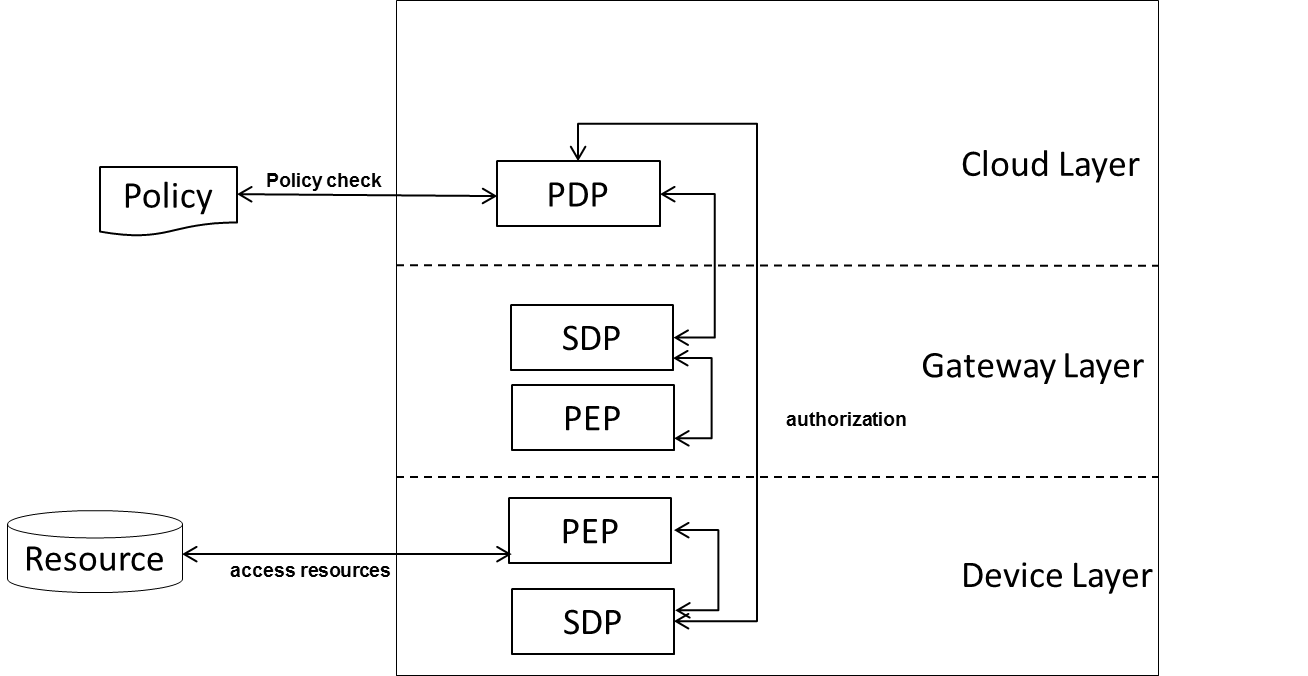
\includegraphics[height=3.5in]{policy.png}
%\caption{Policy based system architecture which allows for effective storage of provenance data}
%\label{policy_architecture}
%\end{center}
%\end{figure}
%
%\section{Provenance Information Flow}
%
%This section unifies components of our IoT provenance collection system. Figure \ref{flow_chart} depicts a flowchart which illustrates how provenance is generated and how storage policy is used to enforce access on provenance data. Input data are represented in green while processes are represented by the blue rectangles. Policy document determines what kinds of provenance data to collect and store. The policy creator can be a device owner who has access and authority to the device. A yaml configuration file is passed as an input to the the tracer component. This contains the barectf application that collects CTF trace from sensor-actuator readings on the device. The yaml configuration is an essential portion of the tracer system. It is used to generate application CTF trace output. It contains instructions of what trace data to collect. The policy framework takes a modular approach: policy component can be added at various layers of the IoT architecture. The policy engine is involved with the authorization and enforcement of policies generated. This portion generates a decision based on the policy evaluation. The response from the policy allows provenance effectively pruned. Provenance data stored as CTF trace in Neo4j, a graph database and is mapped to PROV-JSON format. The PROV-JSON serialization is used as input to our IDS system which serves as the provenance application. Figure \ref{flow_chart} below illustrates the relationship between various component in the provenance aware IoT framework.
%
%\begin{figure}[h!]
%\begin{center}
%
%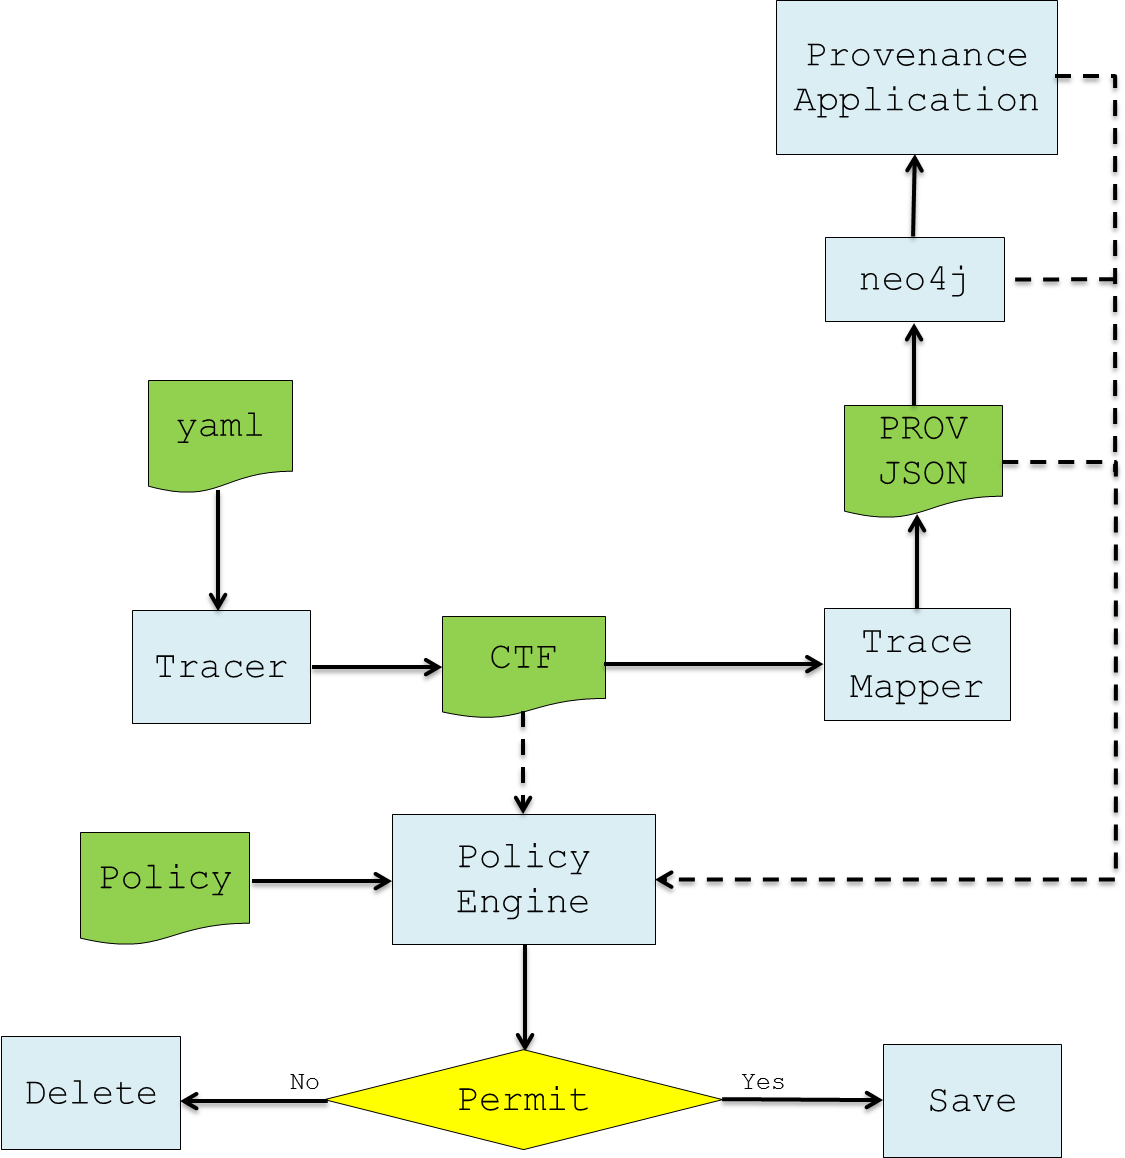
\includegraphics[width =4.5in]{policy_flowchart.PNG}    
%\end{center}
%\caption{Provenance Information Flowchart illustrating how provenance data is generated and how storage policy is used to enforce access on provenance data. }
%\label{flow_chart}
%\end{figure}
%
%\section{Policy-Based System}
%
%In this section, I will explain various software tools in which I plan to use to implement a proof of concept for the policy-based storage system. Some of these tools have been illustrated in chapter 4. 
%
%
%\par To map CTF trace to PROV-DM format, I plan to use babeltrace, a plugin framework that allows converting from one trace format to another. PROV-DM data is represented in PROV-JSON serialized format and stored in a graph database. PROV-JSON is used as input to the provenance application which leverage provenance data to perform some application specific functionality. For our implementation, we choose to use a provenance-based IDS system.
%
%%ProvToolbox, a java library for creating and visualizing provenance data. It also allows the conversion of provenance data from one format to another(e.g PROV-DM to PROV-JSON).
%
%To implement our policy based framework, we plan to use the eXtensible Markup Language (XACML)  \cite{xacml} to generate an enforceable provenance storage policy for our IoT policy based system. XACML is a standard that defines constructs for policy language(i.e policy document, policy enforcement and policy authorization). We employ this standard in building our policy based system.
%
%
%\subsection{Policy-Based Framework Evaluation}
%
%To evaluate the effectiveness of our policy based approach,we utilize the application use case as described in chapter 4. We also use the provenance based IDS, PIDAS as the provenance application. The details of PIDAS is also discussed in chapter 4. To evaluate PIDAS, we analyze the throughput and overhead incurred in addition to false negative and true positive.







%\section{Proposed Research Experiment Evaluation}
%
%We plan to evaluate the effectiveness of our approach for the provenance collection framework and our framework for efficient provenance storage by running an intrusion detection system for IoT device. An IDS is used to detect malicious attacks based on a certain policy or threshold set by an administrator. There are two types of  IDS: Rule-based approach, or anomaly based approach. The rule based approach allows for intrusion monitoring based on rules specified by an administrator. On the other hand, anomaly based IDS which monitors intrusion based on patterns that falls out of the normal system function. Most anomaly\-based approach deals with machine learning to classify normal or anomalous behavior.  

%\begin{definition}
%{\rm By {\em absolute width\/} $W$ of an interval ${\bf x}=[x^-,x^+]$, we mean
%twice the absolute half-width of ${\bf x}$, i.e.,
%$$
%  W([x^-,x^+])=x^+-x^-.
%$$}
%\end{definition}
%
%\begin{definition}
%{\rm We say that an interval ${\bf x}$ is {\em $\Delta$-narrow in the sense
%of absolute accuracy\/} if $W({\bf x})\leq\Delta$.}
%\end{definition}
%
%\begin{definition}
%{\rm Let $\varepsilon>0$ be a real number, let $D\subseteq R^N$ be a closed
%and bounded set of positive $N$-dimension volume $V(D)>0$, and let
%$P(x)$ be a property that is true for some points $x\in D$.  We say that $P(x)$
%is true for {\em $(D,\varepsilon)$-almost all\/} $x$ if}
%$$
%  \frac{V(\{x\in D|\neg P(x)\})}{V(D)}\leq \varepsilon.
%$$
%\end{definition}
%
%\begin{definition}
%{\rm Let $\eta>0$ be a real number.  We say that intervals
%$$
%  [r_1-d_1,r_1+d_1],\ldots,[r_n-d_n,r_n+d_n]
%$$
%are {$\eta$-close} to intervals
%$$
%  [\tilde x_1-\Delta_1,\tilde x_1+\Delta_1],\ldots,[\tilde x_n-\Delta_n,
%   \tilde x_n+\Delta_n]
%$$
%if $|r_i-\tilde x_i|\leq\eta$ and 
%$|d_i-\Delta_i|\leq\eta$ for all $i$.}
%\end{definition}
%
%\begin{definition}
%{\rm Let $\cal U$ be an algorithm that solves some systems of interval linear
%equations, and let $\eta>0$ be a real number.  We say that an algorithm 
%$\cal U$ is {\em $\eta$-exact\/} for the interval matrices ${\bf a}_{ij}$ and
%${\bf b}_i$ if for every interval matrix ${\bf a}_{ij}^\prime$ and 
%${\bf b}_i^\prime$ that are $\eta$-close to ${\bf a}_{ij}$ and ${\bf b}_i$,
%the algorithm $\cal U$ returns the exact solution to the system}
%$$
%  \sum_{j=1}^n {\bf a}_{ij}^\prime x_j = {\bf b}_i^\prime.
%$$
%\end{definition}
%
%\begin{definition}
%{\rm We say that an algorithm $\cal U$ is {\em almost always exact for narrow 
%input intervals\/} if for every closed and bounded set $D\subseteq R^N
%(N=n\cdot m+n)$ there exist $\varepsilon>0$, $\Delta>0$ and $\eta>0$ such
%that, for $(D,\varepsilon)$-almost all $\tilde a_{ij}$ and $\tilde b_i$, if
%all input intervals ${\bf a}_{ij}$ and ${\bf b}_i$
%(containing $\tilde a_{ij}$ and $\tilde b_i$ respectively)
%are $\Delta$-narrow (in the sense of absolute accuracy), then the
%algorithm $\cal U$ is $\eta$-exact for ${\bf a}_{ij}$ and ${\bf b}_i$.}
%\end{definition}
%
%\section{Theorem}
%
%\begin{theorem} \label{almost-all-theorem}
%There exists a feasible (polynomial-time) algorithm $\cal U$ that is almost 
%always exact for narrow input intervals.
%\end{theorem}
%
%\medskip
%
%\noindent
%This theorem was proven in 1995 by Lakeyev and Kreinovich
%(see~\cite{Lakeyev1995}).
%
%\section{Open Problem}
%Theorem \ref{almost-all-theorem} says that we can have a feasible algorithm 
%that solves {\em almost all\/} narrow-interval linear equation systems, but 
%it does not say whether we can solve {\em all\/} of them in reasonable time.  
%Thus, there still remains an open question:
%
%\begin{quote}
%{\it Can a feasible algorithm be developed for the general problem of
%solving systems of linear equations with narrow-interval coefficients?}
%\end{quote}
%
%\noindent
%The answer to this open question is the main concern of this thesis.
%
%We will show that the problem of solving all narrow-interval linear equation
%systems is NP-hard; moreover, we will show that the problem is NP-hard not
%only for intervals that are narrow in the sense of absolute accuracy, but
%also in the sense of relative accuracy.

